\documentclass[11pt]{article}
\usepackage[paper=letterpaper,margin=1in]{geometry}
\usepackage{subfig}
\usepackage{graphicx}
\usepackage{fancyvrb}
\usepackage{upquote}
\usepackage[colorlinks=true, linkcolor=blue, urlcolor=blue, citecolor=blue, anchorcolor=blue]{hyperref}
\usepackage{amsmath}
\usepackage{indentfirst}

\usepackage{tikz}

\title{The LAN Before Time Heartbeat Protocol}
\author{Brandon Ingli \and Dylan Toombs \and Chase Anderson}
\date{\today}

\begin{document}
  \maketitle

  \section{Protocol Design}
  A packet in our protocol consists of a version number, a flag for if the protocol 
  was generated in client/server mode (set) or peer-to-peer mode (cleared), if 
  the packet contains a summary of known heartbeats (set) or just one heartbeat 
  (cleared), the IP address of the sender, reserved space for future use, and 
  the number of heartbeats in the rest of the packet. Each heartbeat contains 
  the IP of the generating machine, the beat number from that machine (starting 
  from zero when the software starts up each time), a timestamp of when the 
  beat was generated (assuming each machine is synchronized on the same 
  timeserver), the Time-to-Live of the heartbeat in seconds, and the time until the next 
  heartbeat is expected to be sent in seconds.

  In client/server mode, a list of IP addresses are provided with server
  priority from top to bottom. The designated "server" sends a summary packet
  containing all known clients' heartbeats including its own. This server is
  designated by receiving packets with the Client/Server flag set and the Is 
  Summary flag cleared (indicating an individual machine's Heartbeat is contained). 
  Once the server dies, the next client on the IP
  list knows to become the new server because it stops receiving the summary
  packet and starts receiving individual beats from other nodes. When a server 
  starts receiving summaries again, it knows to stop sending summaries itself. 
  Every client
  waits from 0 to 30 seconds and then they send their heartbeat to the server.
  Every client has a 30 second TTL while the current server has a TTL of
  90 seconds. The server waits between 0 and 15 seconds to send each summary 
  to the other nodes.

  In peer-to-peer mode, every client just sends all their known heartbeats,
  including their own, to every other client in the list of IP addresses. Similar 
  to a server sending summaries, each node sends its summary to each other 
  node at a random interval from 0 to 15 seconds. After 30 seconds of not 
  receiving a packet from another client the given client is considered dead.
  \begin{figure}[h]
    \centering
    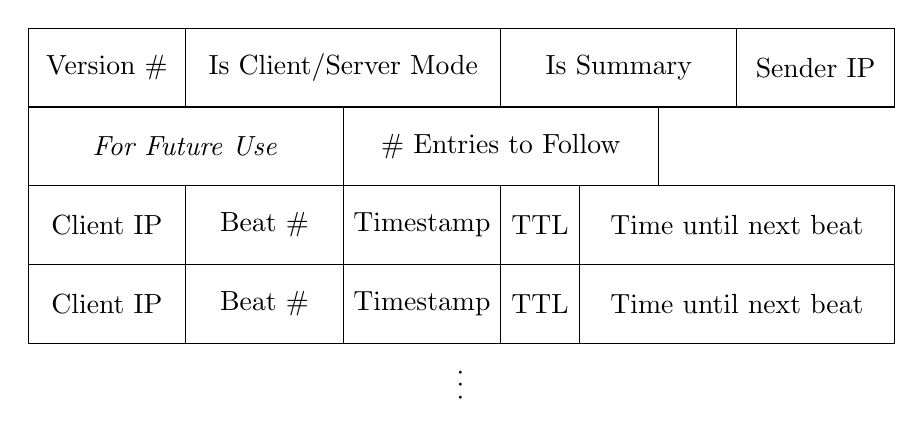
\begin{tikzpicture}

      \draw (0,3) rectangle (2,4);
      \node [anchor=center] at (1,3.5) {Version \#};

      \draw (2,3) rectangle (6,4);
      \node [anchor=center] at (4,3.5) {Is Client/Server Mode};

      \draw (6,3) rectangle (9,4);
      \node [anchor=center] at (7.5,3.5) {Is Summary};

      \draw (9,3) rectangle (11,4);
      \node [anchor=center] at (10,3.5) {Sender IP};


      \draw (0,2) rectangle (4,3);
      \node [anchor=center] at (2,2.5) {\textit{For Future Use}};

      \draw (4,2) rectangle (8,3);
      \node [anchor=center] at (6,2.5) {\# Entries to Follow};


      \draw (0, 1) rectangle (2, 2);
      \node [anchor=center] at (1,1.5) {Client IP};

      \draw (2,1) rectangle (4,2);
      \node [anchor=center] at (3, 1.5) {Beat \#};

      \draw (4,1) rectangle (6,2);
      \node [anchor=center] at (5, 1.5) {Timestamp};

      \draw (6,1) rectangle (7,2);
      \node [anchor=center] at (6.5, 1.5) {TTL};

      \draw (7,1) rectangle (11,2);
      \node [anchor=center] at (9,1.5) {Time until next beat};

      
      \draw (0, 0) rectangle (2, 1);
      \node [anchor=center] at (1,0.5) {Client IP};

      \draw (2,0) rectangle (4,1);
      \node [anchor=center] at (3, 0.5) {Beat \#};

      \draw (4,0) rectangle (6,1);
      \node [anchor=center] at (5, 0.5) {Timestamp};

      \draw (6,0) rectangle (7,1);
      \node [anchor=center] at (6.5, 0.5) {TTL};

      \draw (7,0) rectangle (11,1);
      \node [anchor=center] at (9,0.5) {Time until next beat};

      \node[draw=none, rotate=90] at (5.5, -0.5) {$\cdots$};


    \end{tikzpicture}
    \caption{The LAN Before Time Heartbeat Packet}
    \label{fig:HeartbeatPacket}
  \end{figure}

  \section{Why do we believe this design is good?}
  We feel this is the most optimal design because in client-server it creates a 
  hierarchy of the devices allowing a long line of fail-safes for the primary
  server. Furthermore, in peer-to-peer, since every client holds a list of known
  heartbeats there is always redundancy in place to prevent the loss of any
  data should a client disconnect from the network. Finally, this design showcases 
  how the same protocol design can be used in many applications (Client/Server 
  and Peer-to-Peer) with no changes, including demonstrating this through code 
  by reusing most of the code between the two implementations with no change.

  \section{Implementation Notes}
  This project was implemented using multiple Java \texttt{Thread}s. This 
  allows us to accomplish every task we need to at the same time, while 
  limiting the amount of duplicate code we needed to write. Any attributes 
  needed by each thread are stored in the \texttt{HeartbeatSharedData} data 
  object, a reference to which is shared to each thread.

  \section{A Note from the Team Leader}
  I (BI) want to commend my teammates for taking on this challenge. They had 
  not encountered multithreading in Java before, and were still new to the 
  socket programming concepts. The fact that they took this challenge head on 
  and were excited about learning more is truly remarkable and indicative of 
  the type of learners they are. While their number of contributions may be 
  lower than mine, they put in just as much effort as me and learned quite 
  a bit along the way.

  \section{Contributions}
  Brandon thought up the core design of the protocol and met with Chase and
  Dylan to make the first draft official. Brandon took the position of team
  leader and delegated the project's different Java classes to each member. For 
  a detailed look at contribution history, you can view the commit history on 
  our GitHub repository: \url{https://github.com/brandoningli/cs-470-project1/}. 
  Each member's GitHub username is provided below.
  \begin{itemize}
    \item Brandon (\texttt{brandoningli}) contributed \dots
    \begin{itemize}
      \item \texttt{Heartbeat}
      \item \texttt{HeartbeatPacket}
      \item \texttt{HeartbeatStatusPrinter}
      \item \texttt{HeartbeatSend}
      \item \texttt{HeartbeatDriverClientServer} and \texttt{HeartbeatDriverP2P}
      \item \texttt{Makefile}
      \item Testing Environment
    \end{itemize}
    \item Chase (\texttt{hypeincarnate}) contributed \dots
    \begin{itemize}
      \item \texttt{HeartbeatSharedData}
      \item \texttt{HeartbeatSummarySend}
    \end{itemize}
    \item Dylan Toombs (\texttt{TheMojaveMajin}) contributed \dots
    \begin{itemize}
      \item \texttt{HeartbeatReceive}
      \item Project Documentation
    \end{itemize}
    \item The \texttt{NetIdentity} class was contributed by \texttt{Decoded4620} 
    on StackOverflow and modified by Brandon. They are attributed in the java 
    file as well.
  \end{itemize}

  After all classes were completed the whole team sat down in a video call to
  observe the testing of the protocol to ensure everything ran properly.

  The entire development process is well documented in the GitHub repo. A
  complete set of project cards and descriptions are available on the site 
  under the ``Projects'' tab.

  \section{Usage}
  Run the program using the included JAR files: 
  
  \noindent\texttt{java -jar <Jar Name>.jar <IP File> <IP Prefix>}

  \begin{itemize}
    \item \texttt{<Jar Name>} is either \texttt{lb4theartbeatClientServer} or \texttt{lb4theartbeatP2P} 
      depending on the Implementation you wish to run.
    \item \texttt{<IP File>} is the relative path to a text file of IP addresses, one per 
      line, in server-priority order (primary first) for client-server mode. The 
      current machine's IP \textit{must} be included in this list as well. Order is 
      irrelevant for peer-to-peer mode.
    \item \texttt{<IP Prefix>} is the beginning of the IP address for the network 
      you want to use this protocol with. This helps the program to determine the 
      correct IP address of the local machine. For example, if you're running 
      across Truman's network, use the prefix \texttt{150.243}
  \end{itemize}

  In client/server mode, it is recommended that you start up the primary server 
  first for best results. Once the system is up and running, failover happens 
  automatically. The system should still start up properly if the nodes start 
  up out of order from a cold start, but network traffic may be a bit 
  congested at the onset, settling out over time as the primary server is 
  established.
\end{document}